% Name: Hyperbola and its asymptotes
% Description: The hyperbola x²/a² − y²/b² = 1 with its vertices, its foci at c = √(a² + b²), the box of half-sides a and b, and the asymptotes y = ±(b/a)x through its corners.
% Tags: conic section, hyperbola, asymptotes, foci

\usetikzlibrary{arrows.meta}

\begin{tikzpicture}[>={Stealth}, every node/.style={font=\small}]
  % a = 2, b = 1.5, so c = 2.5; branches drawn as (±a cosh t, b sinh t)
  \draw[->] (-4.8,0) -- (5,0) node[right] {$x$};
  \draw[->] (0,-3.2) -- (0,3.4) node[above] {$y$};
  \draw[dashed, gray] (-2,-1.5) rectangle (2,1.5);
  \draw[dashed, gray!70!black] (-4.4,-3.3) -- (4.4,3.3) node[right] {$y = \tfrac{b}{a}x$};
  \draw[dashed, gray!70!black] (-4.4,3.3) -- (4.4,-3.3) node[right] {$y = -\tfrac{b}{a}x$};
  \draw[very thick, blue!70!black, domain=-1.45:1.45, samples=50] plot ({2*cosh(\x)},{1.5*sinh(\x)});
  \draw[very thick, blue!70!black, domain=-1.45:1.45, samples=50] plot ({-2*cosh(\x)},{1.5*sinh(\x)});
  \foreach \x in {-2.5, 2.5} \fill[orange!85!black] (\x,0) circle (1.8pt);
  \node[below, orange!85!black] at (2.5,0) {$F_2$};
  \node[below, orange!85!black] at (-2.5,0) {$F_1$};
  \foreach \x in {-2, 2} \fill (\x,0) circle (1.5pt);
  \node[below] at (1,0) {$a$};
  \node[left] at (0,0.75) {$b$};
\end{tikzpicture}
